\documentclass{article}
\usepackage{graphicx}

\begin{document}

\begin{enumerate}
    \item The output F of the digital circuit shown can be written in the form(s)\rule{2cm}{0.5pt}
    \begin{figure}[h]
        \centering
        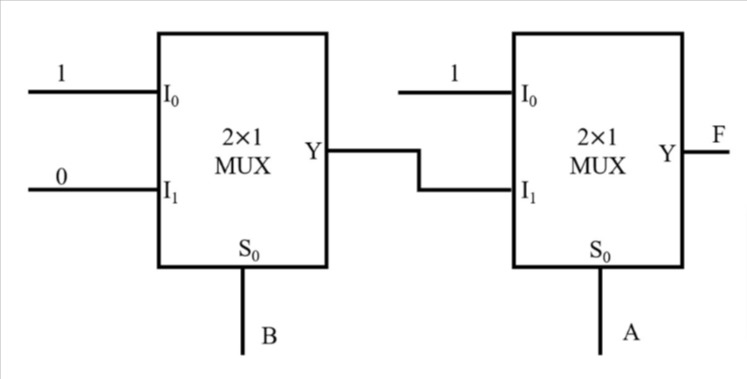
\includegraphics[width=\columnwidth]{gate.jpg}
        \caption{}
        \label{fig:my_label}
    \end{figure}
    \begin{enumerate}
        \item $\overline{A.B}$
        \item $\bar{A}$+$\bar{B}$
        \item $\overline{A + B}$
        \item $\bar{A}$.$\bar{B}$ \hfill (GATE IN 2022)
    \end{enumerate} 
\end{enumerate}
\end{document}
